\documentclass{article}
\usepackage[utf8]{inputenc} %кодировка
\usepackage[T2A]{fontenc}
\usepackage[english,russian]{babel} %русификатор 
\usepackage{mathtools} %библиотека матеши
\usepackage[left=1cm,right=1cm,top=2cm,bottom=2cm,bindingoffset=0cm]{geometry} %изменение отступов на листе
\usepackage{amsmath}
\usepackage{graphicx} %библиотека для графики и картинок
\graphicspath{}
\DeclareGraphicsExtensions{.pdf,.png,.jpg}
\usepackage{subcaption}
\usepackage{pgfplots}
\usepackage{float}

\begin{document}
% НАЧАЛО ТИТУЛЬНОГО ЛИСТА
\begin{center}
    \Large
    Федеральное государственное автономное \\
    образовательное учреждение высшего образования \\ 
    «Национальный исследовательский университет ИТМО»\\
    \vspace{0.5cm}
    \large
    Факультет программной инженерии и компьютерной техники \\
    Направление подготовки 09.03.04 Программная инженерия \\
    \vspace{1cm}
    \Large
    \textbf{Отчёт по лабораторной работе №8} \\
        По дисциплине «Информационная безопасность» ( семестр 7)\\
        Мини-исследование: Утечка данных и цифровая гигиена
    \large
    \vspace{8cm}

    \begin{minipage}{.33\textwidth}
    \end{minipage}
    \hfill
    \begin{minipage}{.4\textwidth}
    
        \textbf{Студент}: \vspace{.1cm} \\
        \ Дениченко Александр Олегович P3412\\
        \textbf{Практик}:  \\
        \ Маркина Татьяна Анатольевна
    \end{minipage}
    \vfill
Санкт-Петербург\\ 2025 г.
\end{center}
\pagestyle{empty}
% КОНЕЦ ТИТУЛЬНОГО ЛИСТА 
\newpage
\pagestyle{plain}

\section*{Задание}

\begin{itemize}
    \item Проверьте свой основной email-адрес на сайте https://haveibeenpwned.com/ (сервис проверяет, не фигурирует ли ваша почта в известных утечках данных). Внимание: Используйте только email! Не вводите здесь свои пароли!
    \item Если ваши данные были найдены, проанализируйте, в каких утечках они фигурируют и какие данные были скомпрометированы (пароли, имена, номера телефонов и т.д.).
    \item Проведите аудит своих публичных данных в социальных сетях (ВК, Telegram и др.). Какая информация о вас доступна незнакомым людям?
    \item На основе проведенного анализа составьте 5-7 личных правил цифровой гигиены (например, "не использовать один пароль на разных сайтов", "проверять настройки конфиденциальности в соцсетях раз в полгода").
\end{itemize}

\section{Проверка основного email-адреса на сайте}

\begin{center}
    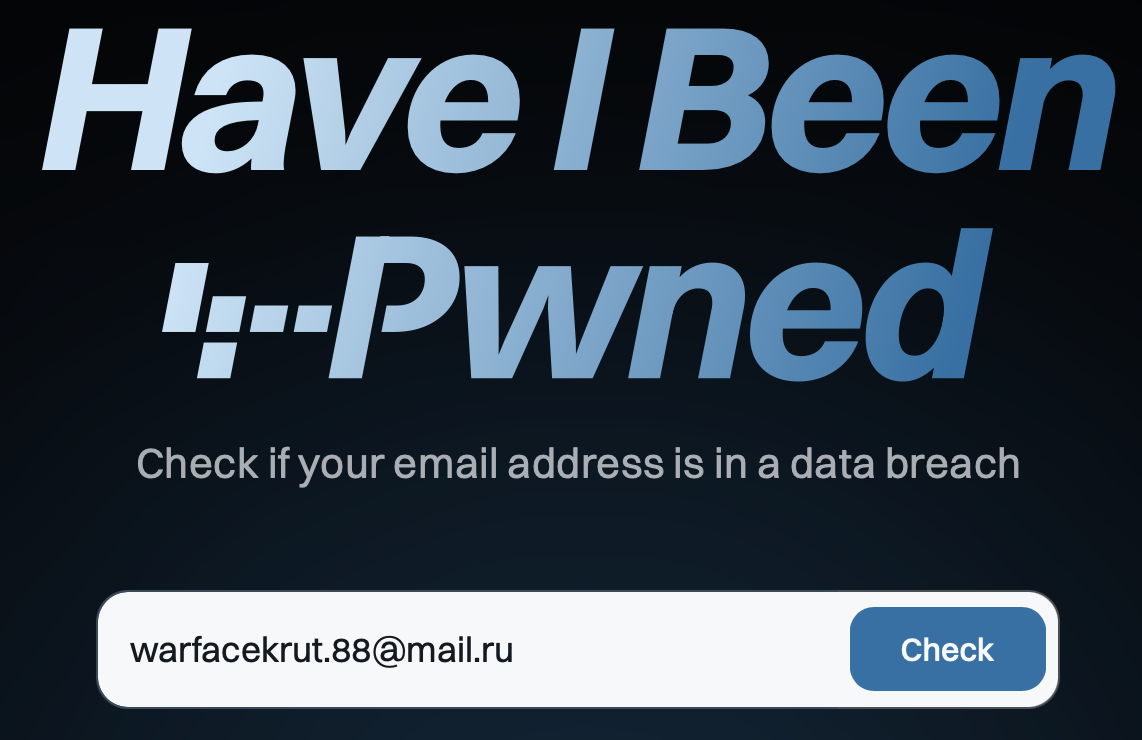
\includegraphics[width=.9\textwidth]{1}
\end{center}
\begin{center}
    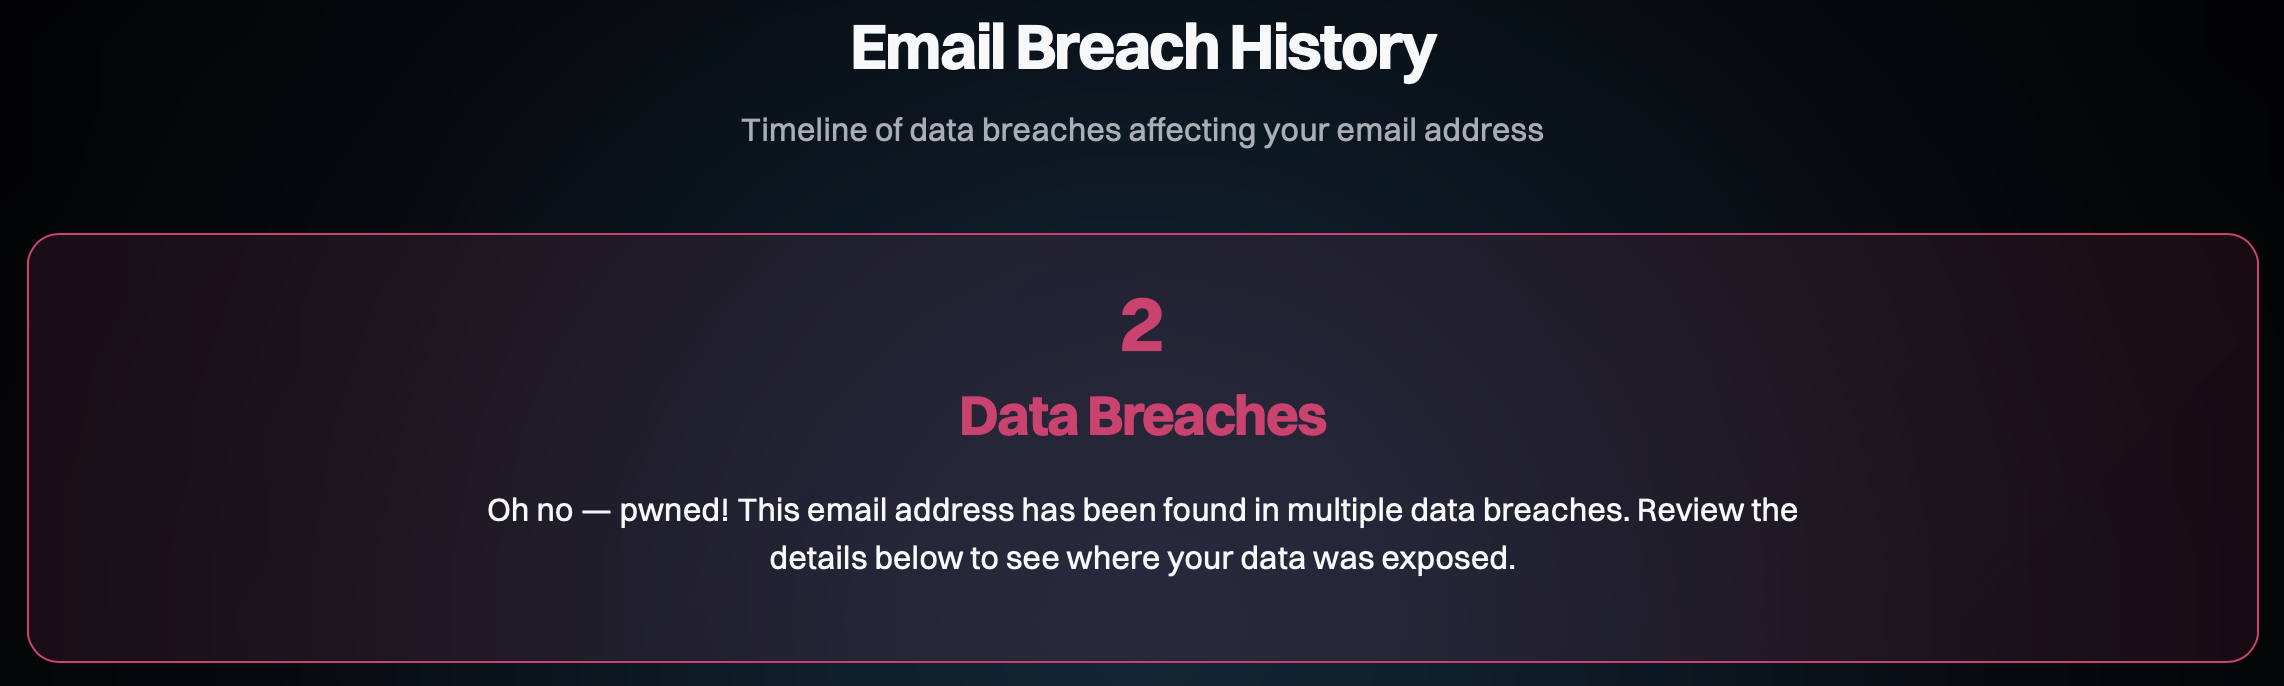
\includegraphics[width=.9\textwidth]{2}
\end{center}

\section{Анализ утечек}

\subsection{Первая утечка}

В январе 2019 года на популярном хакерском форуме была обнаружена большая коллекция списков учетных данных. Сайт показал следующее:

\begin{center}
    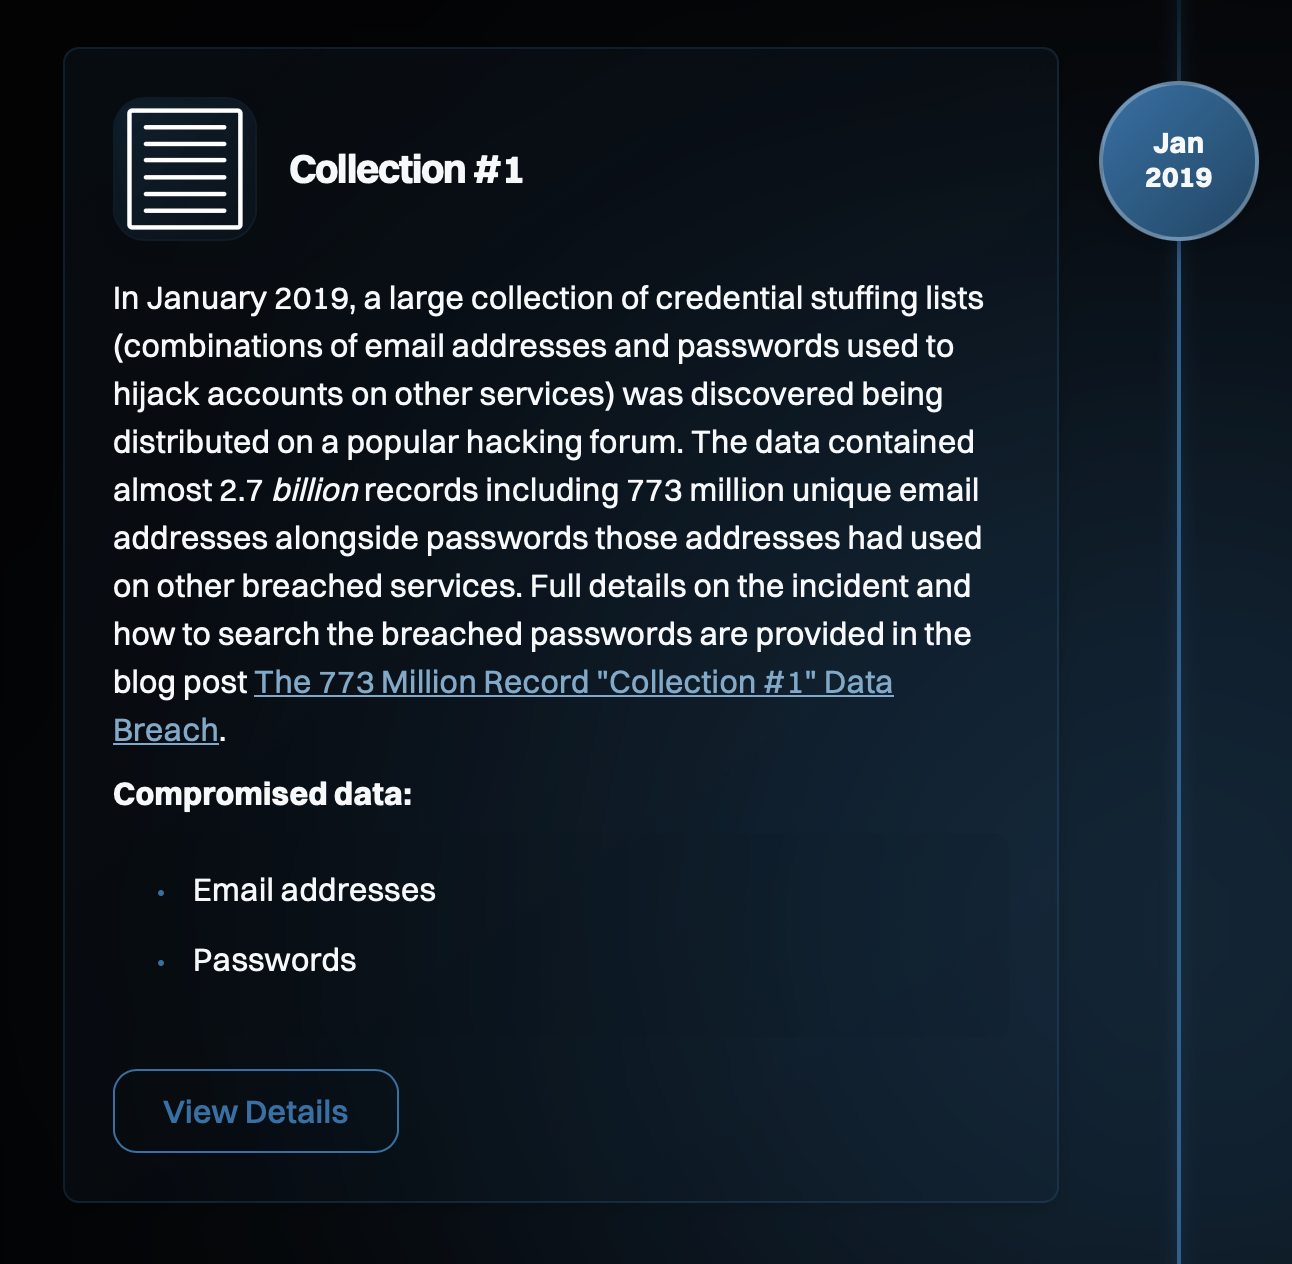
\includegraphics[width=.9\textwidth]{3}
\end{center}

Утечка в которой они фигурируют:

\begin{itemize}
    \item The 773 Million Record "Collection 1" Data Breach
\end{itemize}

Данные которые были скомпрометированы:

\begin{itemize}
    \item Адрес электронной почты
    \item Пароль -- пароль был несколько раз изменён с того момента
\end{itemize}

\textbf{Интересное из статьи:}

В базе содержится 1,160,253,228 уникальных пар email-адрес и пароль, а уникальных email-адресов — 772,904,991


\subsection{Вторая утечка}
В мае 2018 года российский хакерский форум Lolzteam подвергся утечке данных, которая разоблачила 400 тысяч участников. 
Сайт показал следующее:

\begin{center}
    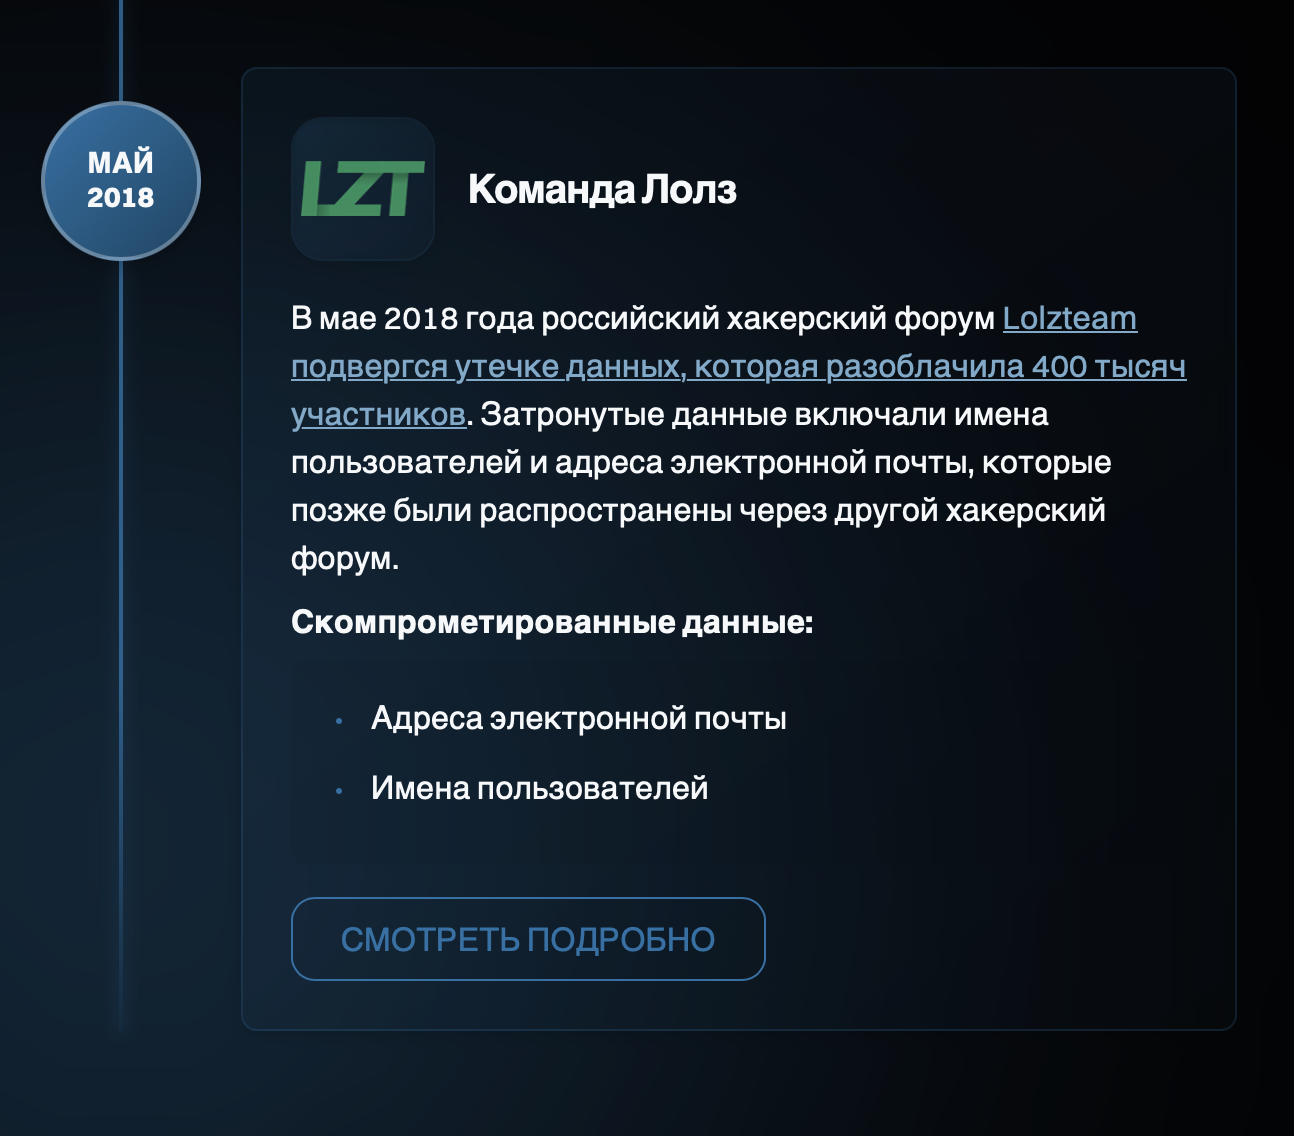
\includegraphics[width=.9\textwidth]{5}
\end{center}

Данные которые были скомпрометированы:

\begin{itemize}
    \item Адрес электронной почты
    \item Имя пользователя
\end{itemize}

\textbf{Интересное из статьи: }

Утечка затронула личные данные более 405 000 участников сообщества Lolzteam.net, включая их email-адреса, номера телефонов, часовые пояса и детали активности. 
Несмотря на масштабную утечку, пароли пользователей в базе не были раскрыты.

\section{Аудит своих публичных данных}

\subsection{VK}

Изначально есть смысл рассмотреть мою страницу от не залогиненного пользователя.
\begin{center}
    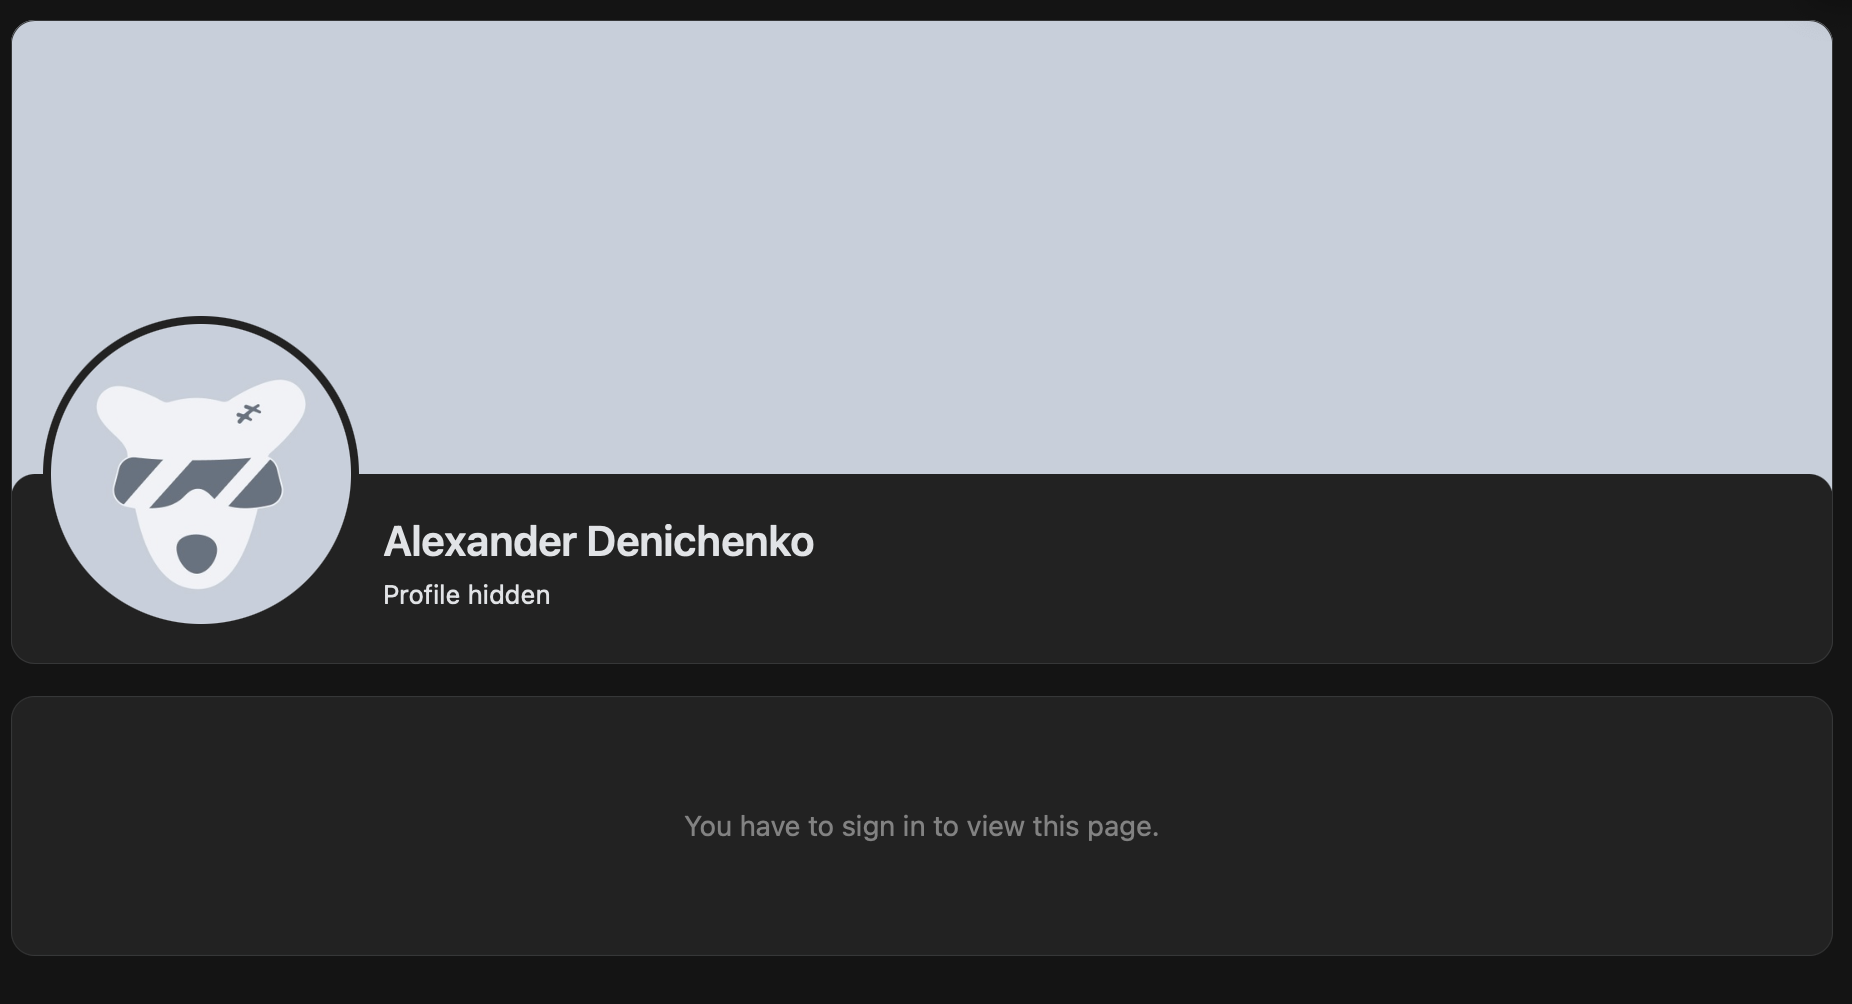
\includegraphics[width=.9\textwidth]{vk}
\end{center}

Итог: такой пользователь ничего не видит, кроме моей Фамилии и Имени.

\begin{center}
    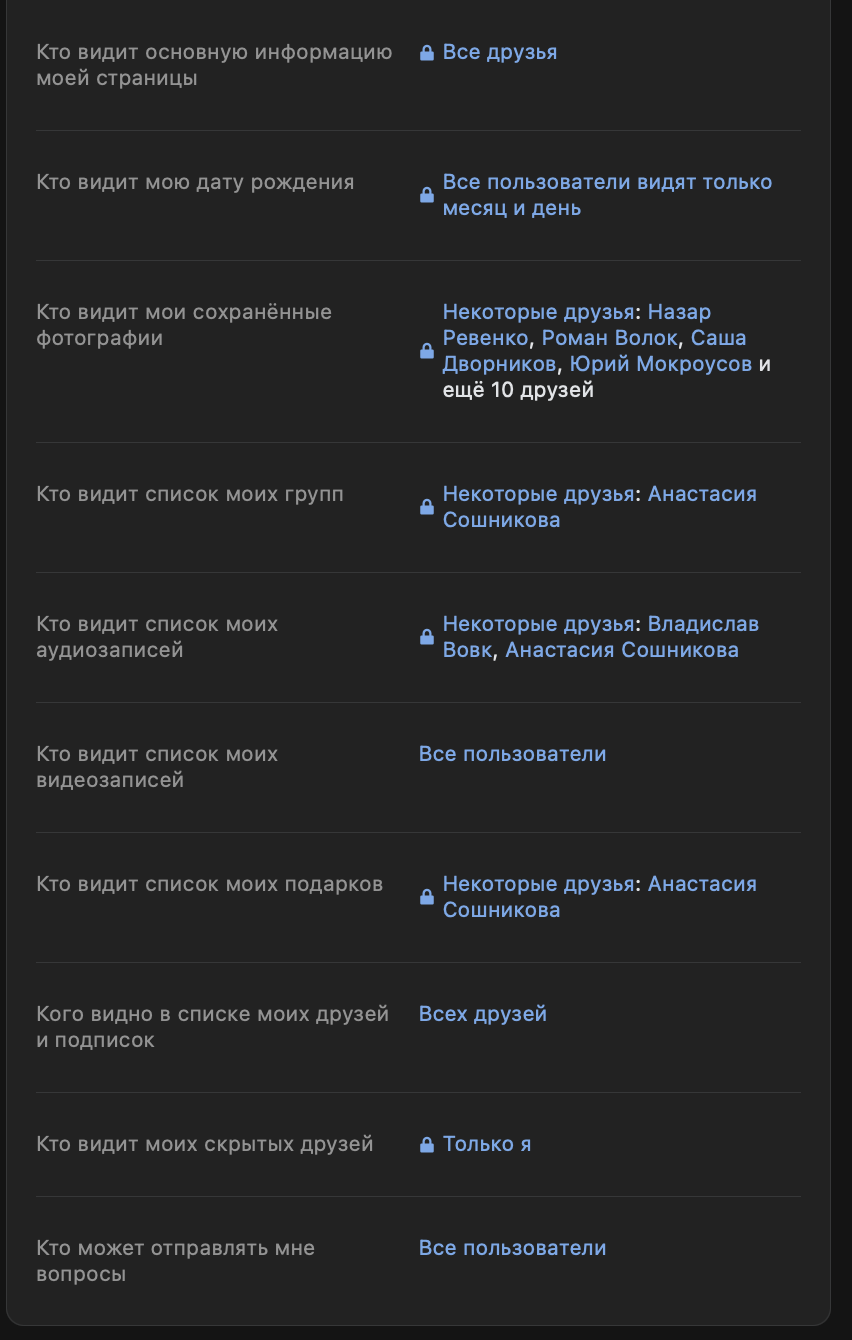
\includegraphics[width=.9\textwidth]{6}
\end{center}
\begin{center}
    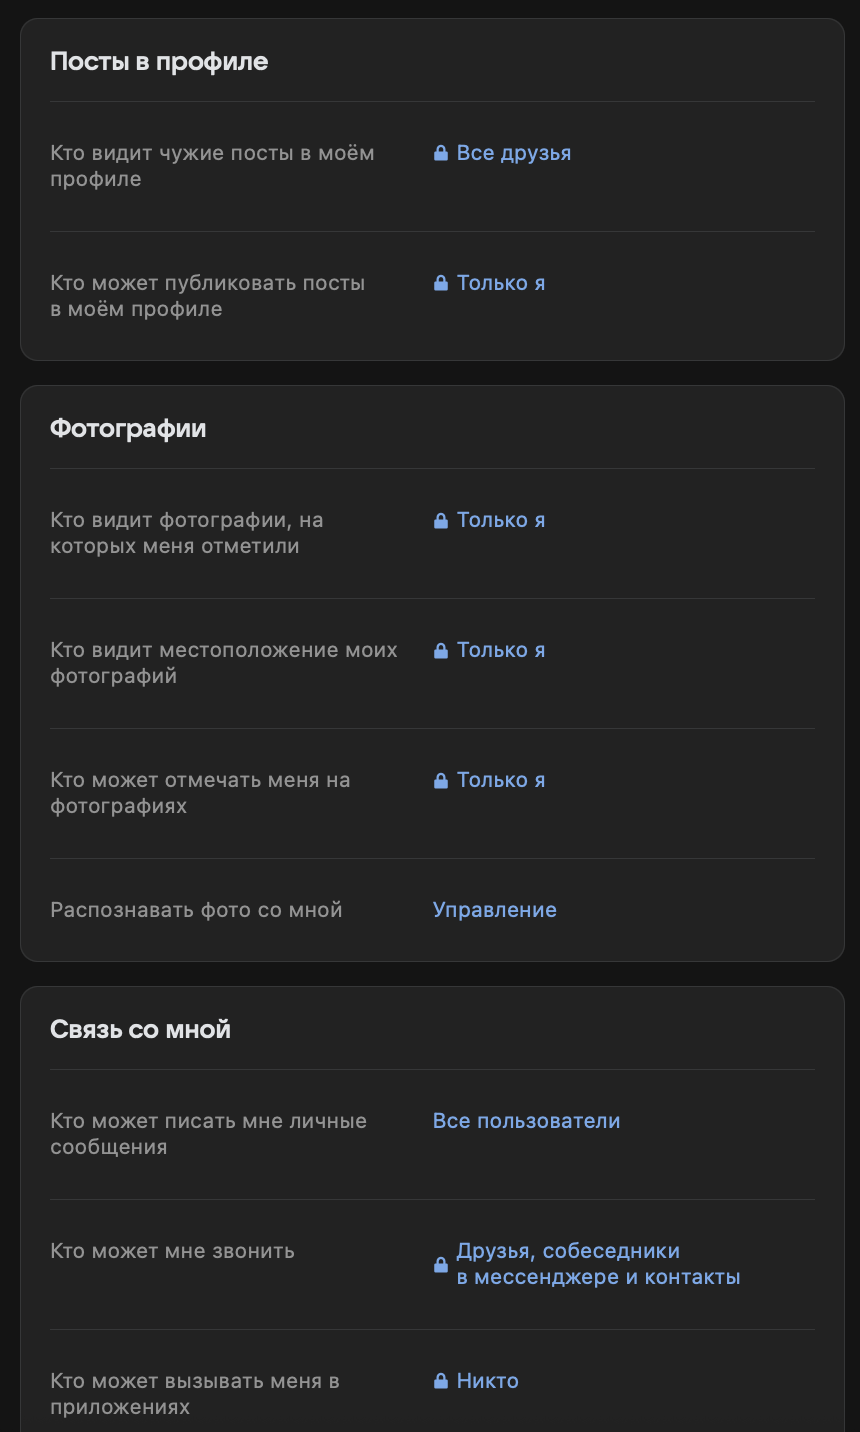
\includegraphics[width=.9\textwidth]{7}
\end{center}
\begin{center}
    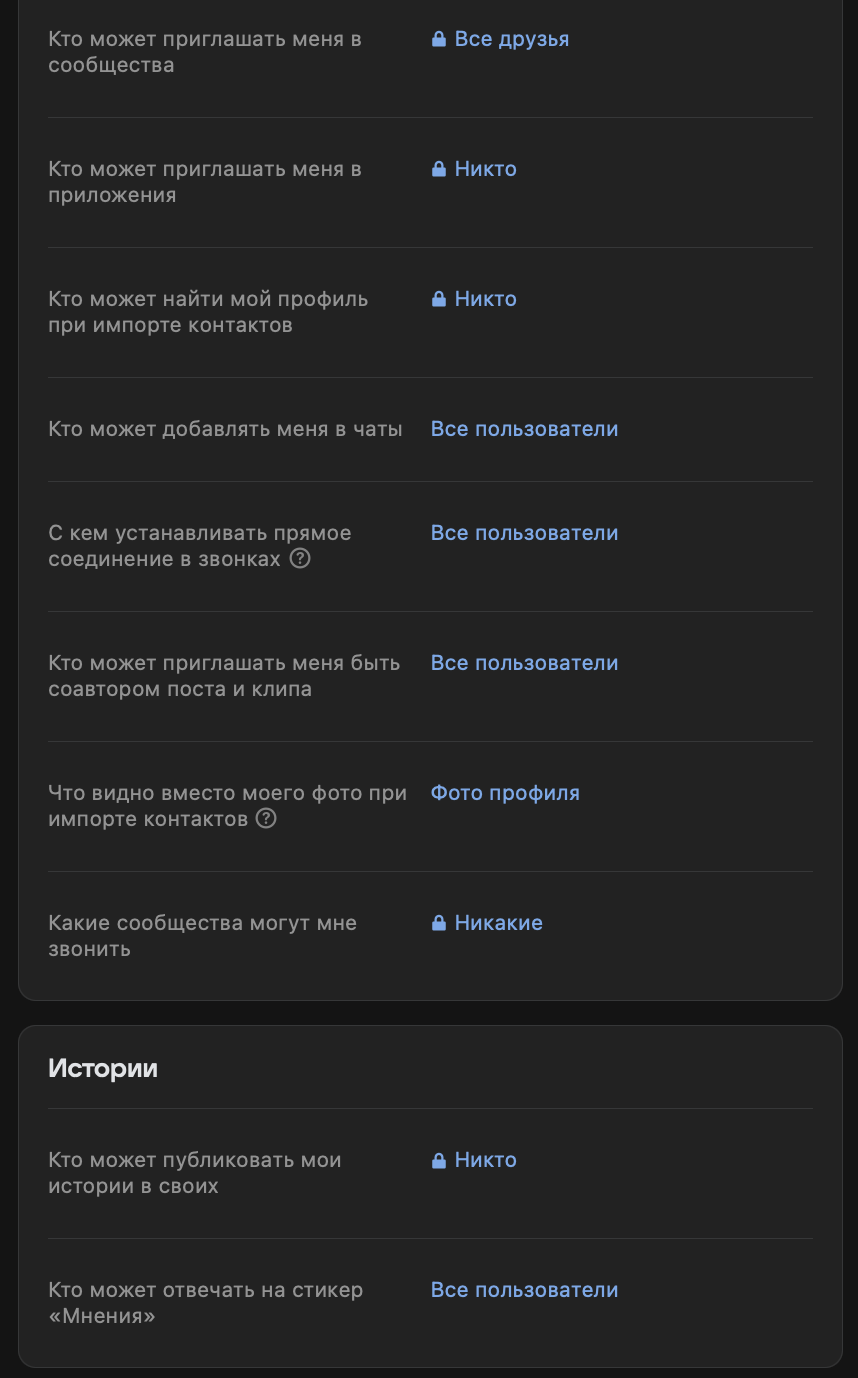
\includegraphics[width=.9\textwidth]{8}
\end{center}
\begin{center}
    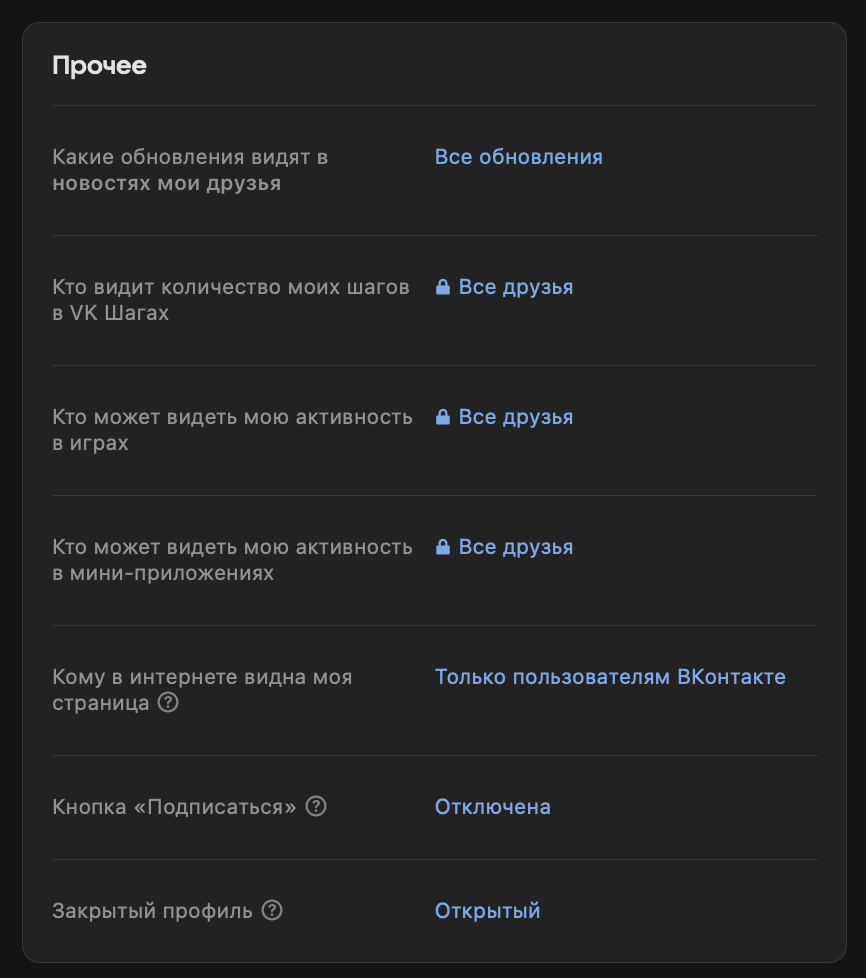
\includegraphics[width=.9\textwidth]{9}
\end{center}

Публичная информация для незнакомцев:

\begin{itemize}
    \item Видят только месяц и день рождения.
    \item Имеют возможность писать мне личные сообщения.
    \item Могут приглашать в чаты, быть соавторами постов/клипов.
    \item Видят список моих видеозаписей.
    \item Возможность найти и просмотреть профиль доступна только зарегистрированным пользователям ВКонтакте.
\end{itemize}

Приватность персональных данных:

\begin{itemize}
    \item Основная информация, список групп, друзей, подписок, подарков, аудиозаписей, сохранённых фото, активность — доступны только друзьям или ограниченному кругу лиц.
    \item Все публикации, фотографии, отметки, местоположение, активность в отметках — доступны исключительно мне.
    \item Чужие посты, публикации на странице, комментарии — доступны только друзьям, публикация разрешена только мне.
    \item Входящие звонки полностью закрыты или доступны только друзьям.
\end{itemize}

Что лучше предпринять:

\begin{itemize}
    \item Для ещё большей безопасности можно закрыть доступ к видеозаписям и заявкам на добавление в чаты для всех, кроме друзей.
\end{itemize}

Касательно безопасности:

\begin{center}
    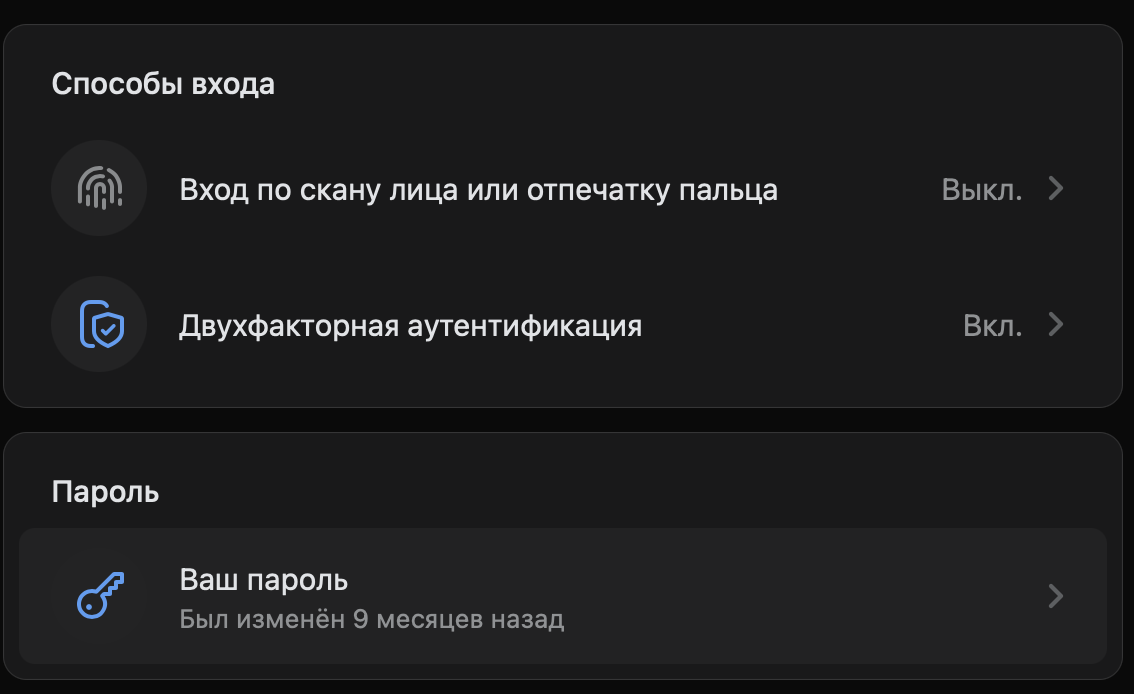
\includegraphics[width=.9\textwidth]{10}
\end{center}

\begin{center}
    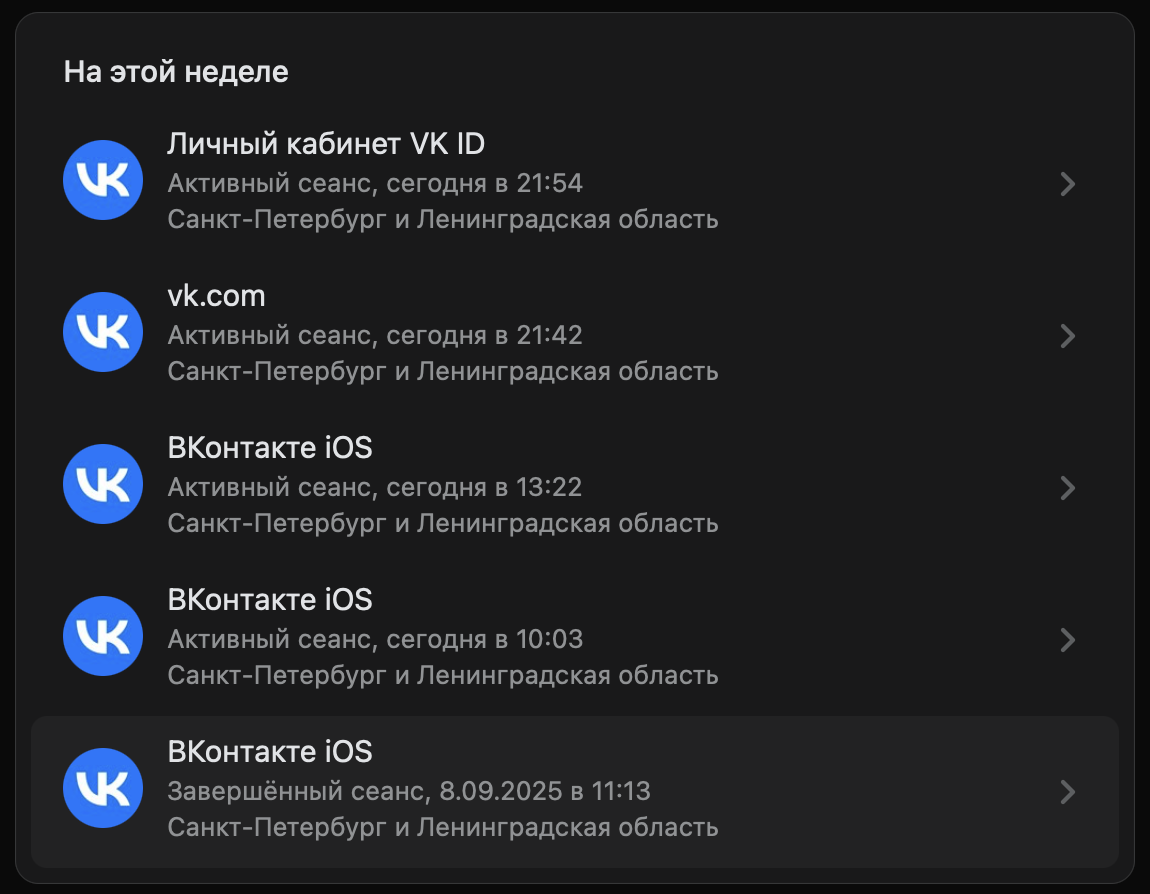
\includegraphics[width=.9\textwidth]{11}
\end{center}

Что лучше предпринять:

\begin{itemize}
    \item Регулярная смена пароля (может быть около 6 месяцев).
    \item Периодически проверять список активных сессий.
\end{itemize}

\subsection{Telegram}

Как меня видят пользователи:

\begin{center}
    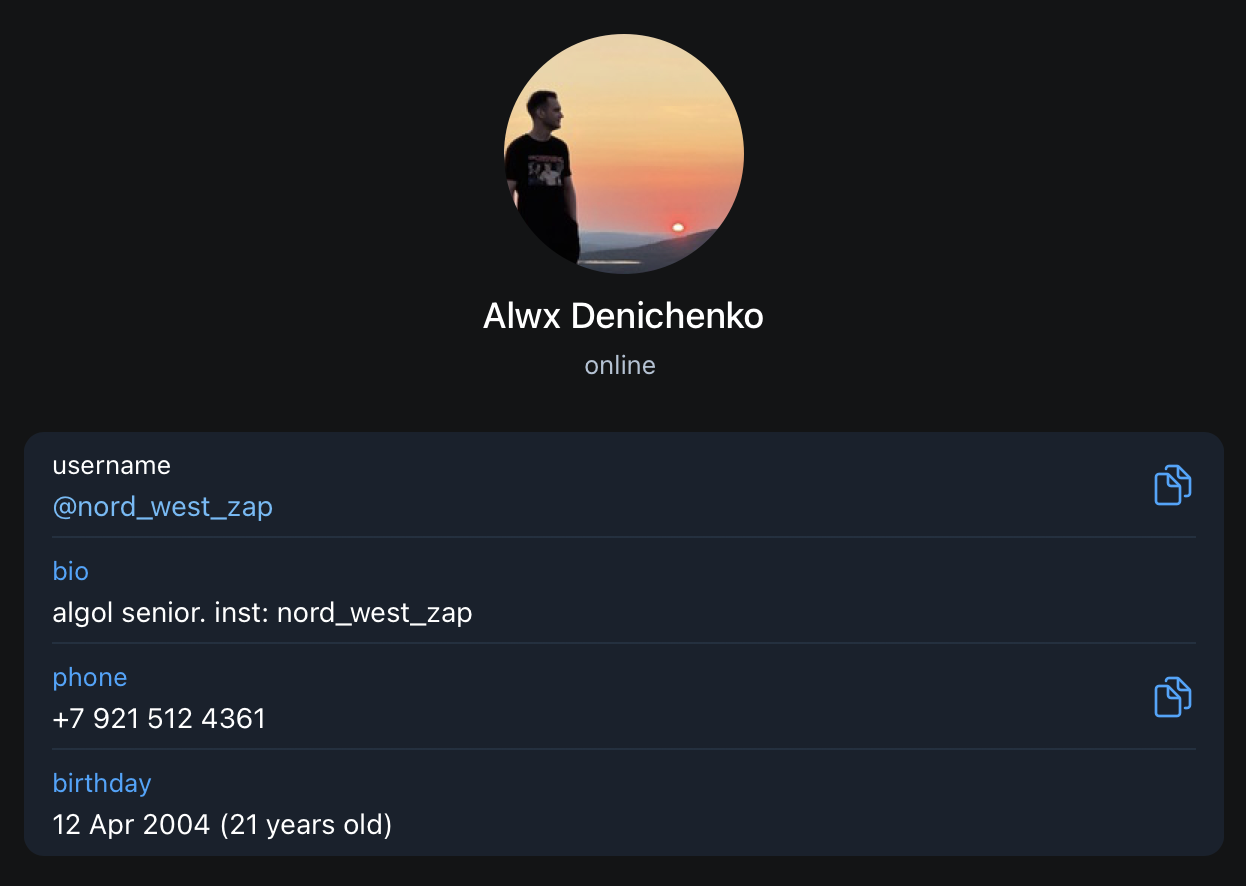
\includegraphics[width=.9\textwidth]{12}
\end{center}

Мои настройки приватности:

\begin{center}
    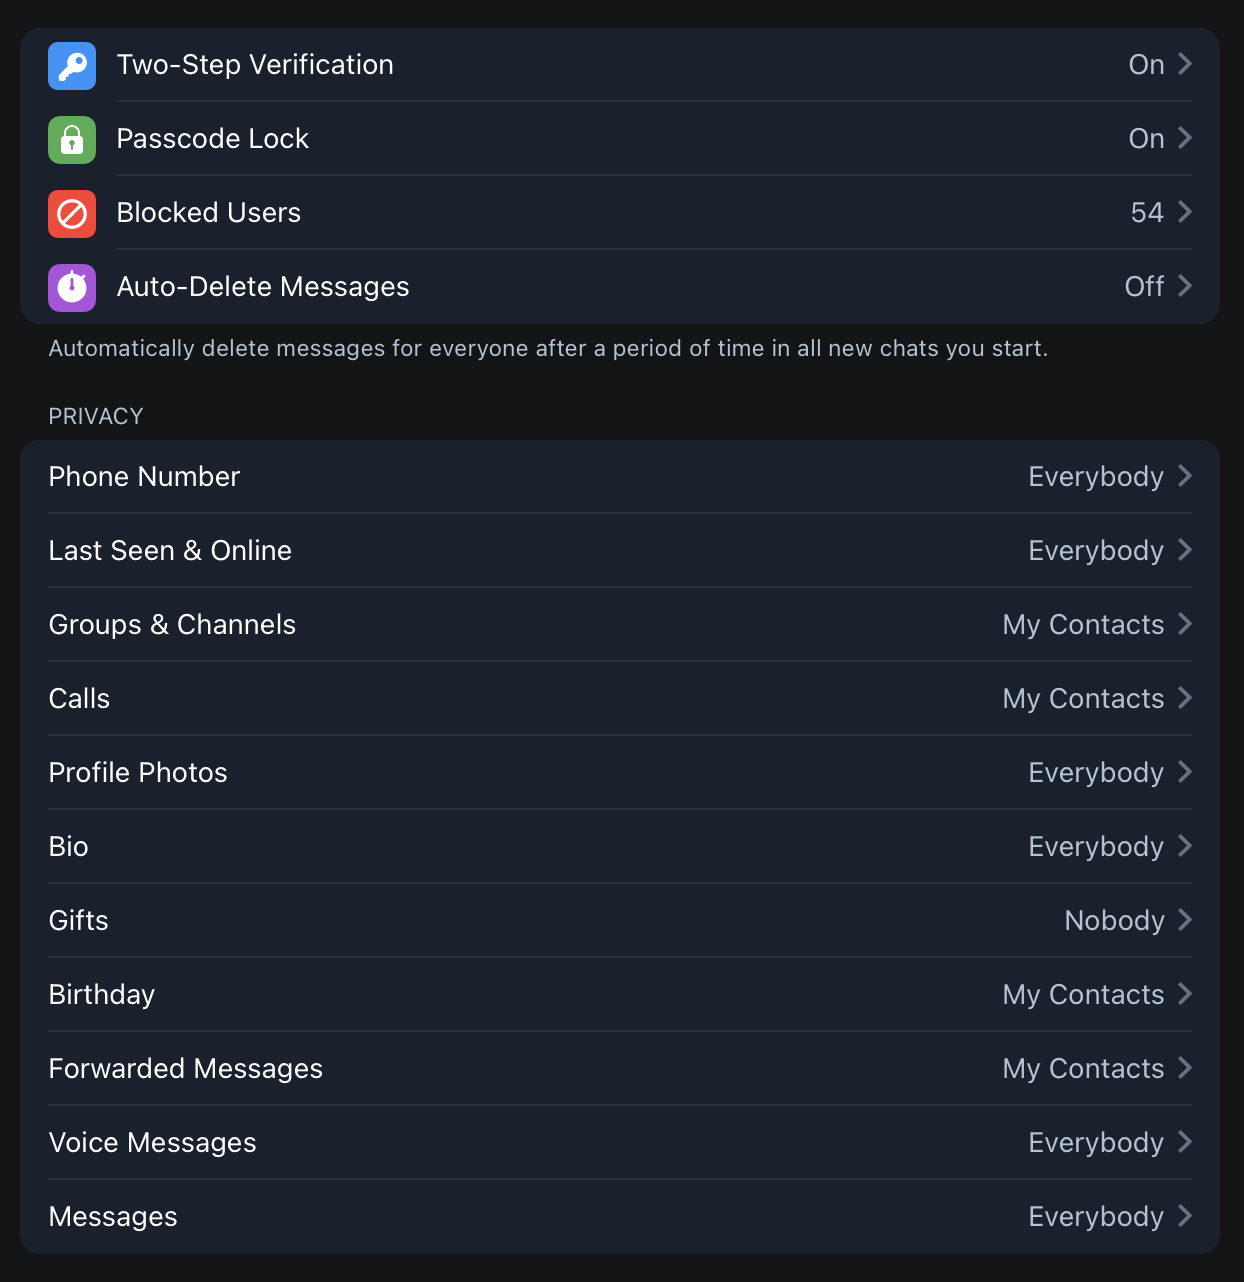
\includegraphics[width=.9\textwidth]{13}
\end{center}
\begin{center}
    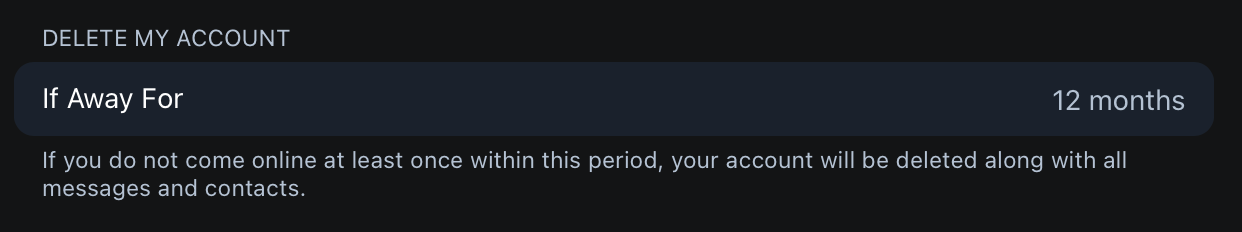
\includegraphics[width=.9\textwidth]{14}
\end{center}

Доступная публично информация:

\begin{itemize}
    \item Имя, username, биография —- всегда видны всем, позволяют быстро идентифицировать. Причём в био указан ещё один контакт.
    \item Телефон —- полностью публичен, что опасно: с этим номером могут пытаться отправить спам, фишинговые сообщения, искать меня на других сервисах.
    \item Дата рождения —- показывается публично, может использоваться при попытках подбора пароля и социальной инженерии.
\end{itemize}

Приватность и безопасность:

\begin{itemize}
    \item Включена двухфакторная аутентификация и код-пароль.
    \item Автоудаление сообщений выключено -- возможно было бы полезно сделать это.
    \item Звонки, пересланные и голосовые сообщения открыты только для контактов.
\end{itemize}

Что лучше предпринять:

\begin{itemize}
    \item Ограничить видимость номера телефона и даты рождения (только контакты или вообще никто).
    \item Профильную фотографию и биографию также лучше показывать только контактам для ограничения круга лиц.
    \item Включить автоудаление сообщений, чтобы повысить конфиденциальность взаимодействий.
\end{itemize}

\section{Правила цифровой гигиены}

На основе проведенного анализа утечек данных и аудита социальных сетей, я вывел для себя следующие правила цифровой гигиены:

\begin{enumerate}
    \item Проводить регулярный аудит настроек приватности в социальных сетях (раз в полгода), особенно проверяя доступность личных данных, таких как номер телефона, дата рождения и другая персональная информация.
    
    \item Использовать двухфакторную аутентификацию на всех платформах, где это возможно, как это уже реализовано в моих аккаунтах Telegram и ВКонтакте (так как у меня был горький опыт с ними)
    
    \item Менять пароли на ключевых сервисах каждые 6 месяцев, учитывая риск компрометации данных, как это случилось в утечке Collection 1.
    
    \item Регулярно проверять список активных сессий во всех социальных сетях и мессенджерах, удаляя неактивные или подозрительные сессии.
    
    \item Ограничить публичную доступность личной информации: настроить видимость номера телефона, даты рождения и других персональных данных только для контактов.
    
    \item Периодически проверять свою электронную почту на сервисах типа haveibeenpwned.com для своевременного выявления случаев утечки данных.
\end{enumerate}


\end{document}
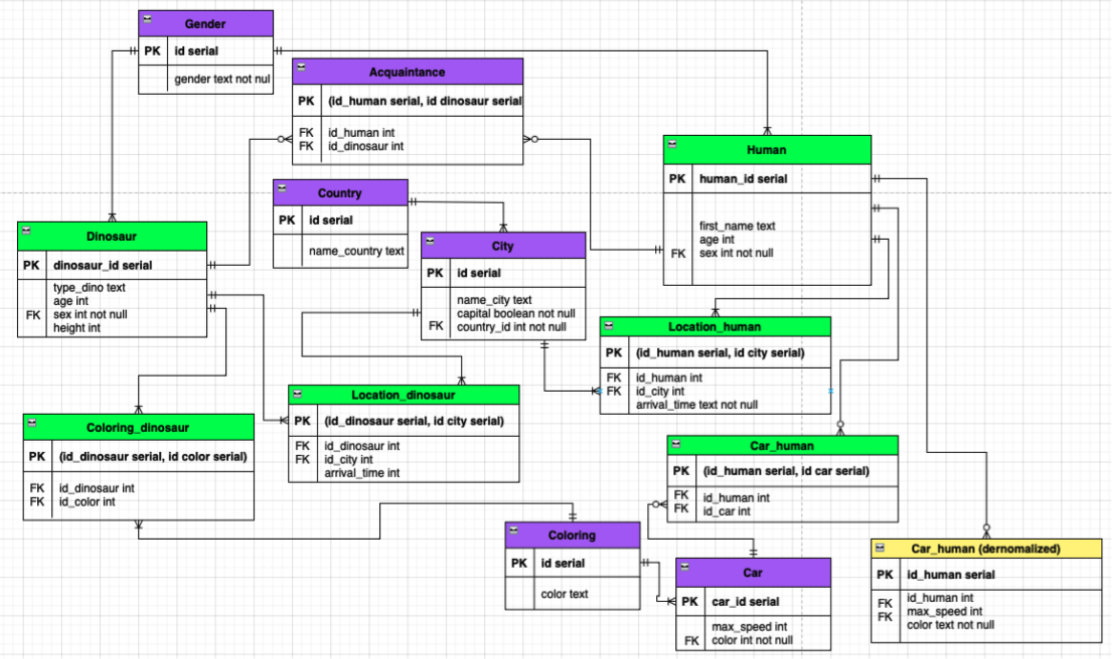
\includegraphics[width=.9\textwidth]{123}